\subsubsection{Fonte de alimentação}

% SLIDE DE FONTE DE ALIMENTAÇÃO
\begin{frame}
\frametitle{Fonte de alimentação}

Para a escolha correta da fonte de alimentação é necessário definir a demanda de energia elétrica que os dispositivos que são alimentados pela fonte necessitam.

Conforme a determinação da tensão de saída e o cálculo de corrente necessária, é possível determinar que a fonte deve ter 12 V e 10,64 A.

\begin{figure}
\centering
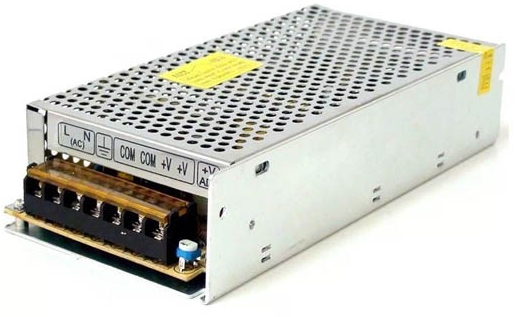
\includegraphics[scale = 0.5]{figs/fonte}
\end{figure}

\end{frame}
